\documentclass{article}
\usepackage[utf8]{inputenc}
\usepackage{amsmath}
\usepackage{graphicx}
\usepackage{hyperref}
\usepackage[english]{babel}\usepackage{subcaption}
\usepackage{sidecap}
\usepackage{lipsum}
\usepackage{multicol}
\usepackage{sectsty}
% \sectionfont{\centering}
\usepackage[a4paper,top=2cm,bottom=2cm,left=2cm,right=2cm]{geometry}
\title{Deep Quaternion Neural Networks for 3D Sound \\ Source Localization and Detection
\\ \large{\vspace{0.4cm}Project of Neural Network Course, Prof. Uncini}}
\author{Sveva Pepe 1743997 \\  Marco Pennese 1749223 \\  Claudia Medaglia 1758095}
\date{}

\begin{document}
    \maketitle
    % \begin{abstract}
    %     We work with 3D audio sounds, in particular we analyze the sound event localization and detection (SELD). 
    %     \\ We were provided with a dataset containing the sounds that were recorded with the first-order Ambisonics microphone. 
    %     These sounds are then represented using spherical harmonics decomposition in the quaternion domain, to then be passed to 
    %     the neural network which will be towed in order to obtain the best possible results in output.
    %     \\ The neural network is quaternion convolutional, with the addition of some recurrent layers.
    %     The aim of the project is to detect the temporal activities of a known set of sound event classes and to further locate them 
    %     in space by using quaternion-valued data processing.
    % \end{abstract}
    \section{Introduction}
    Sound source localization is a fundamental task, expecially in revembrant and multiple sources envoirments.\\
    In this project, we work with 3D audio sounds captured by first-order Ambisonic microphone and these sounds are then represented 
    by spherical harmonics decomposition in the quaternion domain.
    \\ The aim of the project is to detect the temporal activities of a known set of sound event classes and to further locate them in 
    the space using quaternion-valued data processing, in particular we focus on the sound event localization and detection. 
    \\ In order to do this, we use a given Quaternion Recurrent Convolutional Neural Network (QRCNN) 
    for the joint 3D sound event localization and detection (SELD) task.
    % Talk about SELD, which is made up of DOA and SED. Say what I am in a general way, don't go into too much detail, don't go too 
    % far [my advice]. (they are well written in the last paper sent by our friend cominiello).
    % To say that with quaternions the performances are better than without.
    % Then do you.
    % At the end of the introduction, say what the next sections are made up of. 
    \section{Quaternion domain}
    3D audio files are sampled using the Ambisonics technique, where sampling is based on the decomposition of sound in a linear 
    combination of orthogonal bases of spherical harmonics.
    \\ In this project the first-order Ambisonics (FOA) was considered, which is composed of 4 microphone capsules. The first is
    a pressure microphone, the other three are orthogonal eight-shaped microphones related to the pressure gradient, or the acoustic
    speed.
    \\ The pressure microphone is an omnidirectional microphone that has unity gain in all directions. It is indicated by the letter W 
    and corresponds to the spherical harmonic function of order 0.
    Instead the other three microphones are denoted respectively with X, Y, Z and correspond to the harmonic functions of order 1.
    \\ Our goal is to use spherical harmonics in the quaternion domain, so let's consider four ambisonic signals, namely $x_W[n]$, 
    $x_X[n]$, $x_Y[n]$ e $x_Z[n]$, as a single quaternion signal:
    \begin{equation*}
        x[n]=x_W[n]+x_X[n]\hat{i}+x_Y[n]\hat{j}+x_Z[n]\hat{k}
    \end{equation*}
    where x[n] is quaternion-valued ambisonic signal and the four components define the B-Ambisonics format, in fact, we have:
    \begin{equation*}
        \begin{cases}
            x_W[n] = \frac{s[n]}{\sqrt{3}} \\
            x_X[n] = s[n] \cos(\theta) cos(\varphi) \\
            x_Y[n] = s[n] \sin(\theta) cos(\varphi) \\
            x_Z[n] = s[n] \sin(\varphi)
        \end{cases}
    \end{equation*}
    The factor $\frac{1}{\sqrt{3}}$ to the omnidirectional microphone allows to attenuate the average energy of that channel by 
    3 dB about on the full sphere, thus making it equal to the average energy of all the other channels.
    \\ We note that $x_W[n]$ is the real component of the quaternion signal, while the $x_X[n]$, $x_Y[n]$ and $x_Z[n]$ are 
    considered the imaginary components.
    \\ Now we have to derive the quaternion-value input features that will be passed to the network, to do this we need the
    acoustic intensity.
    \\ \\ The vector of acoustic intensity, also called sound field, is produced by average of the sound pressure, $p[n]$, and
    the particle velocity, $v[n]$, over time:
    \begin{equation*}
        I[n]=p[n]v[n]
    \end{equation*}
    In addition, the sound field provides the magnitude and direction of the flow of sound energy.
    \\ Since we are using the representation of quaternions with the B-format Ambisonic we are going to rewrite the sound 
    pressure and speed.
    \\ Sound pressure is defined by the signal captured by the omnidirectional signal, $p[n] = x_W[n]$.
    While the particle velocity is defined by the three orthogonal figure-of-eight microphone signals, $v[n]= \frac{-1}{p_0c\sqrt{3}}$,
    $\begin{bmatrix}
            x_X[n] \\
            x_Y[n] \\
            x_Z[n]
        \end{bmatrix}
    $
    \\ where $p_0$ is the mean density of the air and $c$ is the speed of the sound.
    \\ We express the acoustic intensity in the discrete time-frequency domain in terms of pressure $p[k,n]$ and particle with complex
    velocity $v[k, n]$, where k indicates the index of the frequency bin.
    \\ So the acoustic intensity will be equal to:
    \begin{equation*}
        \begin{matrix}
            I[k,n] = p^*[k,n] v[k,n] \\
            \hspace{1.8cm} = I_a[k,n]+jI_r[k,n]
        \end{matrix}
    \end{equation*}
    where * denotes the complex conjugation.
    \\ $I_a$ and $I_r$ are the two components that make up the acoustic intensity, respectively the active and reactive intensity.
    \\ Active intensity is the time average of the acoustic intensity:
    \begin{equation*}
        I_a [k,n]= \Re\{ p^*[k,n]v[k,n]\} 
    \end{equation*}
    which corresponds to transport of sound energy and whose mean value is non-zero.
    \\ Reactive intensity is defined as the imaginary counterpart of active intensity:
    \begin{equation*}
        I_r [k,n]= \Im \{ p^*[k,n]v[k,n]\} 
    \end{equation*}
    which corresponds to the dissipative energy transport and whose mean value is zero.
    \\ Since the intensity vectors contain the information of theacoustical energy direction of a sound wave, the acoustic intensity
    vector can be directly used for DOA estimation, used in localization.
    \\ In theory, the sound DOA can be estimated as the opposite direction of the active intensity vector. In practice, however, 
    the estimates obtained across all time-frequency bins are inconsistent in reverberant environments.
    \\ Active intensity refers directly to DOA, while reactive intensity indicates whether a given frequency-time bin is dominated
    by sound directed by a single source, opposed to overlapping sources or reverberation. 
    \\ In this way, the active and reactive intensity vectors are both extracted from the spectrogram from each audio channel and 
    are used as separate functions.
    \\ We use both the active and reactive intensity vectors across all frequency bins in the STFT domain as input features,
    in particular,  in order to represent the active and reactive intensity vectors we encapsulate the information in two quaternions. 
    \\  Since we have three components for each intensity vector, we also consider one more channel related to the magnitude of the
    omnidirectional microphone signal in order to improve the performances of the localization task.
    \\ Input features can be expressed by the two quaternions $q_a[k,n]$ and $q_r[k,n]$:
    \begin{equation*}
            \begin{matrix}
                q_a[k,n]=\Re\{x_W^*[k,n]x_W[k,n]\} \\
                \hspace{1cm} + \Re\{x_W^*[k,n]x_X[k,n]\}\hat{i} \\
                \hspace{1cm} + \Re\{x_W^*[k,n]x_Y[k,n]\}\hat{j} \\
                \hspace{1cm} + \Re\{x_W^*[k,n]x_Z[k,n]\}\hat{k} \\
            \end{matrix}
    \end{equation*}
    \begin{equation*}
        \begin{matrix}
            q_r[k,n]=\Im\{x_W^*[k,n]x_W[k,n]\} \\
            \hspace{1cm} + \Im\{x_W^*[k,n]x_X[k,n]\}\hat{i} \\
            \hspace{1cm} + \Im\{x_W^*[k,n]x_Y[k,n]\}\hat{j} \\
            \hspace{1cm} + \Im\{x_W^*[k,n]x_Z[k,n]\}\hat{k} \\
        \end{matrix}
    \end{equation*}
    We normalize each time-frequency bin by its total energy $\epsilon_T=\epsilon_P+\epsilon_K$, where $\epsilon_P=|x_W[k, n]|^2$ 
    is the potential energy density related to the sound pressure and $\epsilon_K=\frac{1}{3}(|x_X[k, n]|^2+|x_Y[k, n]|^2+|x_Z[k, n]|^2)$ 
    is the kinetic energy density related to the particle velocity.
    \\ Now can we express the normalize quaternion inputs as:
    \begin{equation*}
        \overline{q}_a [k,n] = \frac{q_a[k,n]}{\epsilon_T} 
    \end{equation*}
    \begin{equation*}
        \overline{q}_r [k,n] = \frac{q_r[k,n]}{\epsilon_T} 
    \end{equation*}
    The proposed model receives the quaternion ambisonic recording, from which it extracts the spectrogram in terms of magnitude and phase
    components using a Hamming window of lengthvM, an overlap of 50\%, and considering only the $\frac{M}{2}$ positive frequencies without the 
    zeroth bin. herefore, from the two quaternion inputs, we obtain afeature sequence of T frames, with an overall dimension of $Tx\frac{M}{2}x8$.
    % What are quaternions, and their connection with 3D audio recorded with Ambisonic.
    % Enter the mathematical formula on the composition (that of the real part + imaginary part).
    % A minimum of considerations on active and reactive intensity, in particular
    % the role of active and reactive intensity in DOA.
    % \\ Formulas of the two "input features" with quaternions.
    \section{Network Structure}
    The model receives as input the quaternions, from which it extracts the spectrogram in terms of magnitude and phase components 
    using a Hamming window.
    \\ The network is a Quaternion Convolutional Recurrent Neural Network (QCRNN).
    In particular, we have three convolutional layers based on quaternions (QCNN), two recurrent layers (QRNN) and finally two parallel 
    outputs, both are composed of two fully-connected layers, which obviously differ in their activation functions and size that 
    receive input from previous layers.
    \\ The QCNN layers are composed of P filter kernels with size $3x3x8$. 
    \\ The three convolutional layers (QCNN) consist of 3 stages: Convolutional, Detector and  Pooling.
    \\ The first stage consists of the convolutional process to the inputs. Since these are quaternions, the convolutional process 
    consists of Hamilton's product:
    \begin{equation*}
        \begin{matrix}
            W \otimes x =(W_wx_w - W_xx_x - W_yx_y - W_zx_z ) \\
               \hspace{1.2cm} + (W_wx_x + W_xx_w + W_yx_z - W_zx_y )\hat{i} \\
               \hspace{1.2cm} + (W_wx_y - W_xx_z + W_yx_w + W_zx_x )\hat{j} \\
               \hspace{1.2cm} + (W_wx_z + W_xx_y - W_yx_x - W_zx_w )\hat{i}
        \end{matrix}
    \end{equation*}
    where x is the vector of the quaternions taken as input and W a generic quaternion filter matrix.
    \\ Hamilton product allows quaternion neural networks to capture internal latent relations within the features of a quaternion.
    \\ After it is applied the Batch Normalization, a technique for improving the speed, performance, and stability of artificial 
    neural networks. It is used to normalize the input layer by adjusting and scaling the activations.
    Also, batch normalization allows each layer of a network to learn by itself a little bit more independently of other layers.
    \\ The second phase concerns the choice of the activation function, which in the case of the three quaternion convolutional layer 
    is the ReLU.\footnote{ReLU stands for rectified linear unit, and is a type of activation function. Mathematically, it is defined 
    as $y = \max(0, x)$ where y is the output and x is the input.}
    \\ For a generic quaternion dense layer we have:
    \begin{equation*}
        y = \alpha( W \otimes x + b)
    \end{equation*}
    where  y is the output of the layer, b is the bias offset and $\alpha$ is quaternion activation function.
    \\ Indeed,  $\alpha(q) = f(q_w) + f(q_x) + f(q_y) + f(q_z)$, q is a generic quaternion and f is rectified linear unit (ReLU) 
    activation function. As we can see, The ReLU is applied to both the real and imaginary part of the quaternion.
    \\ \\ The last stage is the one related to Pooling. Pooling decrease the computational power required to process the data through 
    dimensionality reduction. Furthermore, it is useful for extracting dominant features which are rotational and positional invariant,
    thus maintaining the process of effectively training of the model. In our network we use MaxPooling.
    MaxPooling is done by applying a max filter to non-overlapping subregions of the initial representation.
    \\ Max-pooling is applied along the frequency axis for 
    dimensionality reduction while preserving the sequence length T, we obtain in the end that the output of the 3 QCN has 
    dimension T x 8P and fed to bidirectional QRNN layers to better catch the time progress of the input signals.  
    \\ The network also uses the Dropout technique, which consists in randomly removing network units with some probability $\beta$.
    \\ \\ QRNN are recurring neural networks based on quaternions.
    The peculiarity of recurrent neural networks is that they differ from feedforward nets because they include a feedback loop,
    whereby output from step n-1 is fed back to the net to affect the outcome of step n, and so forth for each subsequent step.
    \\ In these QRNN Q nodes of quaternion gated recurrent units (QGRU) are used in each layer and as a function of activation
    a hyperbolic tangent (tanh).
    \\ \\ The output of the recurrent layer is shared between two fully-connected layer branches each producing the SED as 
    multi-class multilabel classification and DOA as multi-output regression; together producing the SELD output.
    \begin{figure}[htb!]
        \centering
        \fbox{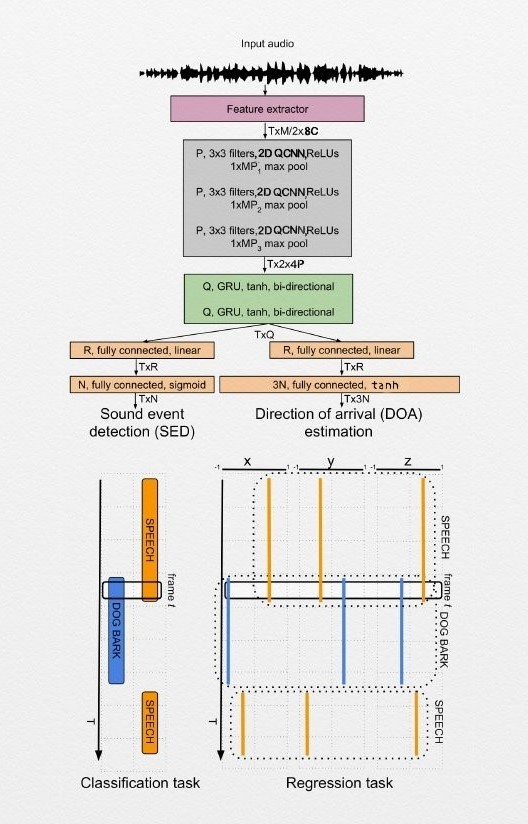
\includegraphics[width=0.5\linewidth]{QRCNN}}
        \label{fig:dqnn}
    \end{figure}
    \\ \\ 
    \subsection{Weight Initialization}
    The appropriate and correct initialization of the network parameters in the quaternion domain must take into account the
    interactions between quaternion-valued components,  thus a simple random and component-wise initialization may result in an 
    unsuitable choice. 
    \\ A possible solution maybe derived by considering a normalized purely quaternion  $u^\triangleleft$ generated for each weight w 
    by following a uniform distribution in $[0,1]$. 
    \\ Each weight can be written in a polar form as:
    \begin{equation*}
        w= |w|e^{u^\triangleleft \theta} = |w| (\cos{\theta} + u^\triangleleft \sin{\theta}) 
    \end{equation*}
    from which it is possible to derive the quaternion-valued components of w:
    \begin{equation*}
        \begin{cases}
            w_W = \phi \cos{(\theta)} \\
            w_X = \phi u_X^\triangleleft\sin{(\theta)} \\
            w_Y = \phi u_Y^\triangleleft\sin{(\theta)} \\
            w_Z = \phi u_Z^\triangleleft\sin{(\theta)}
        \end{cases}
    \end{equation*}
    where $\theta$ is randomly generated in the range $[-\pi, \pi]$ and $\phi$ is a randomly enerated variable related to the variance
    of the quaternion weight, defined as var(W) = $E\{|W|\} - (E\{|W|\})^2 $. where  the second term is null due to the symmetric distribution
    of the weight around 0. Since W follows a Chi distribution with four degrees of freedom, the variance can be expressed as:
    \begin{equation*}
        var(W)=E\{|W|^2\}= \int_0^\infty w^2f(w) dw = 4 \sigma^2
    \end{equation*}
    being $\sigma$ the standard deviation. The variable $\phi$ can be randomly generated in the range $[-\sigma, \sigma]$.
    % Explain the architecture, then start with the 3 QCNN, what is a convolutional network with quaternions 
    % (weights, Hamilton product etc.), which does BatchNormalization (to be specified that this is not based on quaternions), 
    % the activation functions, what is MaxPooling (just explain what it does) and conclude with the Dropout (technique that serves 
    % blah blah blah).
    % \\ Then explain the 2 QRNN recurrent layers and then what a recurrent layer is and the relationship with quaternions, very short.
    % \\ Finally say that the output of the network is doubled, making it possible to do both detection and localization. 
    % Explain the outputs with both two fully-connected layers (remember to specify the activation functions to identify that the two 
    % "outputs" are different).
    % \\I would put image of the network.
    % \\We can also specify the dimensions of the fetures after the QCNN, the QRNN and the FC.
    \section{Dataset}
    The dataset, what it is made of, and how it was divided by us. How many files each subfolder is made up of.
    \section{Metrics}
    The metrics used, therefore the average, SELD SCORE, the confidence interval and I do not know whether to consider the F1 score as well. Obviously with formulas 
    \section{Experiments}
    Our experiments, then the changes we made, the results that come to us, the various graphs.
    Let's see what comes out of it, and in case I would make comparisons with the results that have been obtained from the various papers that have provided us.
    \section{Conclusion}
    The conclusions regarding the project carried out and you have had results based on the metrics that we used.
\end{document}